\documentclass[11pt]{article}
\usepackage{amsmath}
%\usepackage{extsizes}
\usepackage{amsmath,amssymb}
%\usepackage{omegavn,ocmrvn}
%\usepackage[utf8x]{inputenc}
\usepackage[utf8]{vietnam}

\usepackage{longtable}
\usepackage{answers}
\usepackage{graphicx}
\usepackage{array}
\usepackage{pifont}
\usepackage{picinpar}
\usepackage{enumerate}
\usepackage[top=3.0cm, bottom=3.5cm, left=3.5cm, right=2.5cm] {geometry}
\usepackage{hyperref}


\newtheorem{bt}{Câu}
\newcommand{\RR}{\mathbb R}
\Newassociation{sol}{Solution}{ans}
\newtheorem{ex}{Câu}
\renewcommand{\solutionstyle}[1]{\textbf{ #1}.}
\newcommand{\m}[1]{
	\begin{bmatrix}
		#1 
	\end{bmatrix}
}

\newcommand{\Verb}[1]{
\begin{verbatim}
	#1
\end{verbatim}
}

\begin{document}
% \noindent
\begin{tabular*}
{\linewidth}{c>{\centering\hspace{0pt}} p{.7\textwidth}}
Trường ĐHKHTN, ĐHQGHN & {\bf Học Kỳ 2 (2020-2021)}
\tabularnewline
K63 TTƯD & {\bf Tiểu luận cuối kỳ \\ DEADLINE: 12:00 ngày 03/07/2021}
\tabularnewline
\rule{1in}{1pt}  \small  & \rule{2in}{1pt} %(Due date:)
\tabularnewline

%  \tabularnewline
%  &(Đề thi có 1 trang)
\end{tabular*}
%
% \Opensolutionfile{ans}[ans1]

\begin{bt} Cho 1 hệ điều khiển có hàm truyền là 
	\[
	G(s) = \m{\dfrac{s}{(s-1)^2} & \dfrac{s}{s-1} \\ \dfrac{s^2+2s-9}{(s-1)(s+3)} & \dfrac{s+4}{s+3} }
	\]
	a) Hãy đi tìm hai nhận dạng chính tắc điều khiển được và chính tắc quan sát được của hàm truyền trên bằng cả lý thuyết lẫn thực hành lập trình. \\
	b) Áp dụng lệnh sẵn có \verb|minreal| trong $MATLAB/OCTAVE$ cho 2 nhận dạng ở trên, hãy đi tìm nhận dạng tối thiểu.  \\
	c) Sử dụng hệ nhận dạng tối thiểu ở trên, hãy tìm phép đổi biến số thích hợp để chia tỉ lệ (magnitude scaling) sao cho tất cả các biến trạng thái $x_i(t)$ đều có độ lớn bằng với độ lớn tối đa của đầu ra $y(t)$. \\
	d) Nếu mọi tín hiệu đều phải nằm trong phạm vi $\pm10$ V và nếu hàm đầu vào là hàm bước nhảy (step với độ lớn $a$) thì $a$ tối đa có thể là bao nhiêu? 	
\end{bt}


\begin{bt} 
Xét động cơ điện một chiều gắn với tải quay có mômen quán tính $J$ thông qua hộp số có tỷ số truyền $N$ và chịu mômen nhiễu ngoài $T_d$. 

\begin{figure}[h!]
	\centering
	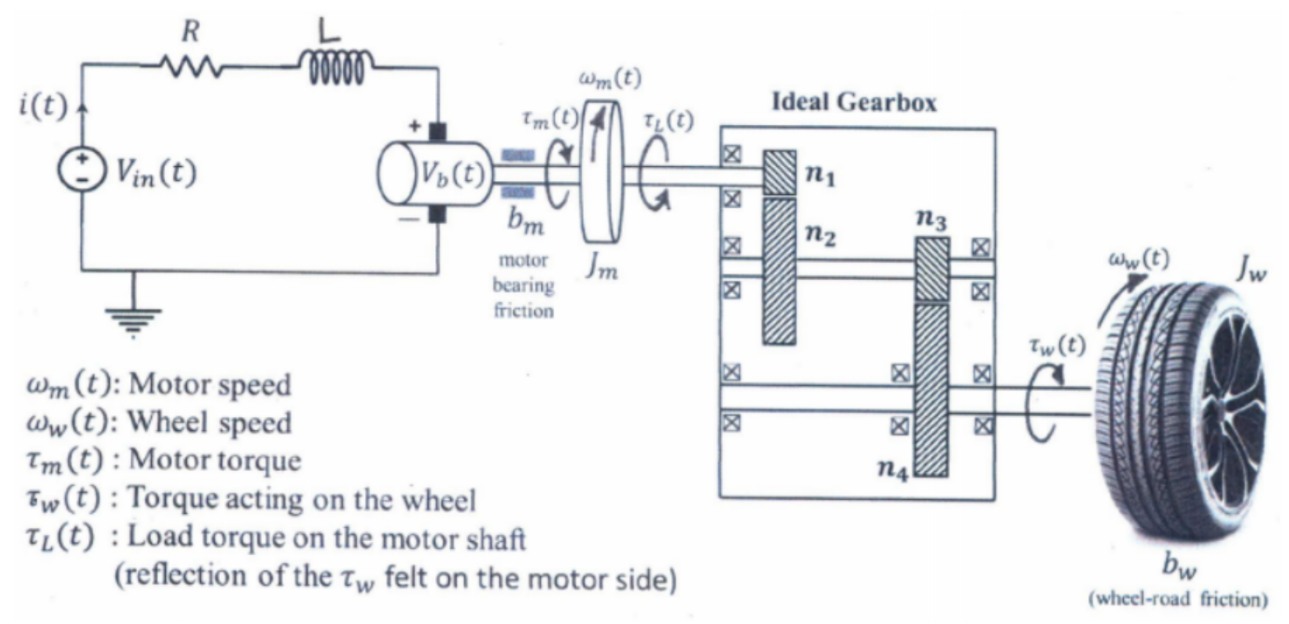
\includegraphics[width=0.7\linewidth]{dcmotor}
	\caption{}
	\label{fig:dcmotor}
\end{figure}

Phương trình chuyển động của hệ được mô tả bằng 
hệ phương trình
%
\begin{align}
& J_e \ddot{\theta}(t) = N K_m i(t) - T_d(t), \\
& L \dfrac{di(t)}{dt} + R i(t) = v(t) - N K_m \dot{\theta}(t),
\end{align}
%
trong đó $\theta(t)$, $\dot{\theta}(t)$, $\ddot{\theta}(t)$ lần lượt là vị trí góc của tải, vận tốc và gia tốc, $J_e = J + N^2 J_m$ là mômen quán tính tương đương quy về phía tải, $J_m$ là mômen quán tính của rôto, $v(t)$ là điện áp đầu vào phần ứng, $i(t)$ là dòng điện chạy qua các cuộn dây phần ứng, $R$ và $L$ lần lượt là điện trở và độ tự cảm của phần ứng rôto và $K_m$ là hằng số emf (suất điện động trở lại).\\

a) Cho các biến trạng thái là $x_1 = \theta$, $x_2 = \dot{\theta}$ và $x_3=i$. Xây dựng mô hình không gian-trạng thái của hệ thống khi đầu ra mong muốn là vị trí góc của tải $\theta$. \\

\textbf{Trong các câu dưới đây ta cho các giá trị cụ thể  $K_m = 0,05$ Nm/A, $R = 1,2$ $\Omega$, $L = 0,05$ H,  $J_m = 0,0008$ $kg/m^2$, $J = 0,02$ $kg/m^2$ và $N = 12$. Sử dụng mô hình vừa tìm được trong câu a), hãy lập trình (copy phần lập trình vào bài (nhớ thay đổi font phần code) \& ghi rõ kết quả cuối cùng vào bài) để thực hiện các nhiệm vụ sau.} \\

b) Tìm hàm truyền của hệ, tìm các cực, không điểm của hệ. \\

c) Sử dụng hàm đầu vào $u$ là hàm xung và hàm bước nhảy hãy vẽ đồ thị của hàm phản hồi trạng thái 0 (với 2 hàm đầu vào trên) trong khoảng thời gian $[0,20]$. \\

d) Ước lượng gần đúng cực đại, cực tiểu của đầu ra trong khoảng thời gian $[0,20]$, với $u$ là hàm bước nhảy. Tìm thời điểm $t$ mà ở đó đầu ra đạt cực trị. \\

e) Mô phỏng hoạt động của hệ thống (chạy code/vẽ hình/mô tả biến động của đầu ra theo thời gian $t$) với điều kiện ban đầu bằng không ($x(0)=0$), $T_d = 0$ và 
đầu vào điện áp được mô tả bởi $v(t) = 3$ V, $0 \leq t \leq 2 $ giây và $v(t) = -3$ V, $2 \leq t \leq 4$ giây, sử dụng lệnh lsim của Matlab/Octave 
với bộ giải ode45. So sánh kết quả mô phỏng.
\end{bt}


\centerline{———————————Hết——————————-}

\end{document}


